\documentclass[12pt]{article}
\usepackage{amsmath, amssymb}
\usepackage{geometry}
\usepackage{hyperref}
\usepackage{booktabs}
\usepackage{array}
\usepackage{tikz}
\usetikzlibrary{arrows.meta, shapes.geometric}

\geometry{margin=1in}
\hypersetup{colorlinks=true, linkcolor=blue, urlcolor=blue}

\title{
    \textbf{CS 440: Introduction to Artificial Intelligence}\\
    \large Assignment 3 --- Probabilistic Reasoning
}
\author{
    Sadhana Vasanthakumar (RUID: 233000133, NetID: sv903)\\
    Sonakshi Sharma (RUID: 229005962, NetID: ss4910)\\
    Simone S Chanekar (RUID: 217006428, NetID: ssc183)
}
\date{Due: April 24, 2026}

\begin{document}

\maketitle
\tableofcontents
\newpage

%%%%%%%%%%%%%%%%%%%%%%%%%%%%%%%%%%%%%%%%%%%%%%%%%%%
\section{Problem 1 (15 points): Bayesian Network}
%%%%%%%%%%%%%%%%%%%%%%%%%%%%%%%%%%%%%%%%%%%%%%%%%%%

The Bayesian network contains five Boolean variables $A$ through $E$.
$A$, $B$, and $C$ are root nodes; $D$ depends on $A$ and $B$; $E$ depends on $B$ and $C$.

\[
P(A=T)=0.2,\quad P(B=T)=0.5,\quad P(C=T)=0.8
\]

\begin{center}
\begin{tabular}{ccc}
\toprule
$A$ & $B$ & $P(D=T \mid A,B)$\\
\midrule
F & F & 0.9\\
F & T & 0.6\\
T & F & 0.5\\
T & T & 0.1\\
\bottomrule
\end{tabular}
\qquad
\begin{tabular}{ccc}
\toprule
$B$ & $C$ & $P(E=T \mid B,C)$\\
\midrule
F & F & 0.2\\
F & T & 0.4\\
T & F & 0.8\\
T & T & 0.3\\
\bottomrule
\end{tabular}
\end{center}

The joint probability factorizes as:
\[
P(A,B,C,D,E)=P(A)\cdot P(B)\cdot P(C)\cdot P(D\mid A,B)\cdot P(E\mid B,C)
\]

\subsection*{(a) All five variables simultaneously true}

\begin{align*}
P(A,B,C,D,E)
  &= P(A)\cdot P(B)\cdot P(C)\cdot P(D\mid A{=}T,B{=}T)\cdot P(E\mid B{=}T,C{=}T)\\
  &= 0.2\times0.5\times0.8\times0.1\times0.3 = \boxed{0.0024}
\end{align*}

The probability that all five Boolean variables are simultaneously true is \textbf{0.0024}.

\subsection*{(b) All five variables simultaneously false}

$P(D{=}F\mid A{=}F,B{=}F)=1-0.9=0.1$ and $P(E{=}F\mid B{=}F,C{=}F)=1-0.2=0.8$:

\begin{align*}
P(\neg A,\neg B,\neg C,\neg D,\neg E)
  &= 0.8\times0.5\times0.2\times0.1\times0.8 = \boxed{0.0064}
\end{align*}

The probability that all five Boolean variables are simultaneously false is \textbf{0.0064}.

\subsection*{(c) $P(\neg A \mid B,C,D,E)$}

Using the normalization trick with
$\alpha=\tfrac{1}{P(A,B,C,D,E)+P(\neg A,B,C,D,E)}$:

\[
P(\neg A\mid B,C,D,E)
  =\frac{P(\neg A,B,C,D,E)}{P(A,B,C,D,E)+P(\neg A,B,C,D,E)}
\]

The numerator uses $P(D{=}T\mid A{=}F,B{=}T)=0.6$ from the CPT:

\begin{align*}
P(\neg A,B,C,D,E)
  &= 0.8\times0.5\times0.8\times0.6\times0.3 = 0.0576
\end{align*}

\[
P(\neg A\mid B,C,D,E)
  =\frac{0.0576}{0.0024+0.0576}
  =\frac{0.0576}{0.0600}
  =\boxed{0.96}
\]

Given that $B$, $C$, $D$, and $E$ are all true, there is a \textbf{96\% probability that $A$ is false}.
The high prior $P(\neg A)=0.8$ combined with the favorable $P(D{=}T\mid\neg A,B{=}T)=0.6$
drives this result.

\newpage
%%%%%%%%%%%%%%%%%%%%%%%%%%%%%%%%%%%%%%%%%%%%%%%%%%%
\section{Problem 2 (15 points): Burglary Network}
%%%%%%%%%%%%%%%%%%%%%%%%%%%%%%%%%%%%%%%%%%%%%%%%%%%

\subsection*{(a) $P(\text{Burglary}\mid\text{JohnsCalls}=T,\text{MaryCalls}=T)$}

\[
P(B)=0.001,\quad P(E)=0.002
\]

\begin{center}
\begin{tabular}{cccc}
\toprule
$B$ & $E$ & $P(A{=}T\mid B,E)$ & $P(A{=}F\mid B,E)$\\
\midrule
T & T & 0.95 & 0.05\\
T & F & 0.94 & 0.06\\
F & T & 0.29 & 0.71\\
F & F & 0.001 & 0.999\\
\bottomrule
\end{tabular}
\qquad
\begin{tabular}{cc}
\toprule
$A$ & $P(J{=}T\mid A)$\\
\midrule
T & 0.90\\
F & 0.05\\
\bottomrule
\end{tabular}
\qquad
\begin{tabular}{cc}
\toprule
$A$ & $P(M{=}T\mid A)$\\
\midrule
T & 0.70\\
F & 0.01\\
\bottomrule
\end{tabular}
\end{center}

With $\alpha=\tfrac{1}{P(J,M)}$, marginalizing over $E$ and $A$:

\[
P(B\mid J,M)
=\alpha\,P(B)\sum_{E}P(E)\sum_{A}P(A\mid B,E)\,P(J{=}T\mid A)\,P(M{=}T\mid A)
\]

The inner sum over $A$ evaluates to:

\begin{center}
\begin{tabular}{ccccc}
\toprule
$B$ & $E$ & $A{=}T$ term & $A{=}F$ term & $f(B,E)$\\
\midrule
T & T & $0.95\times0.9\times0.7=0.598500$ & $0.05\times0.05\times0.01=0.000025$ & $0.598525$\\
T & F & $0.94\times0.9\times0.7=0.592200$ & $0.06\times0.05\times0.01=0.000030$ & $0.592230$\\
F & T & $0.29\times0.9\times0.7=0.182700$ & $0.71\times0.05\times0.01=0.000355$ & $0.183055$\\
F & F & $0.001\times0.9\times0.7=0.000630$ & $0.999\times0.05\times0.01=0.000500$ & $0.001130$\\
\bottomrule
\end{tabular}
\end{center}

\paragraph{For $B=T$:}
\begin{align*}
P(B{=}T,J,M)
  &=\alpha\times0.001\times\bigl[0.002\times0.598525+0.998\times0.592230\bigr]\\
  &=\alpha\times0.001\times[0.001197+0.591046]\\
  &=\alpha\times0.001\times0.592243
   =0.000592\,\alpha
\end{align*}

\paragraph{For $B=F$:}
\begin{align*}
P(B{=}F,J,M)
  &=\alpha\times0.999\times\bigl[0.002\times0.183055+0.998\times0.001130\bigr]\\
  &=\alpha\times0.999\times[0.000366+0.001128]\\
  &=\alpha\times0.999\times0.001494
   =0.001493\,\alpha
\end{align*}

\paragraph{Normalization:}
\[
\alpha=\frac{1}{0.000592+0.001493}=\frac{1}{0.002085}\approx479.6
\]
\begin{align*}
P(B{=}T\mid J,M)&=479.6\times0.000592\approx0.284\\
P(B{=}F\mid J,M)&=479.6\times0.001493\approx0.716
\end{align*}
\[
\boxed{P(\text{Burglary}\mid J{=}T,M{=}T)=\langle\,0.284,\;0.716\,\rangle}
\]

Given that both John and Mary called, there is approximately a \textbf{28.4\% chance a burglary occurred},
and a 71.6\% chance it did not. This matches the result from the textbook.

\subsection*{(b) Chain network: enumeration vs.\ variable elimination}

\paragraph{Enumeration.}
Summing over all $2^{n-2}$ assignments to $X_2,\ldots,X_{n-1}$, each requiring
$n$ multiplications, gives total work $\mathcal{O}(2^n)$ --- exponential in $n$.

\paragraph{Variable elimination.}
Starting from the right end of the chain:
\[
P(X_1\mid X_n{=}T)=\alpha\,P(X_1)\cdots\sum_{x_{n-2}}P(x_{n-2}\mid x_{n-3})
\underbrace{\sum_{x_{n-1}}P(x_{n-1}\mid x_{n-2})\,P(X_n{=}T\mid x_{n-1})}_{f_{X_{n-1}}(x_{n-2})}
\]
Summing out $X_{n-1}$ produces a factor over one variable, reducing to a chain
of length $n-1$. Each of the $n-2$ elimination steps costs constant work, giving
total complexity $\mathcal{O}(n)$ --- \textbf{exponentially faster} than enumeration.

\newpage
%%%%%%%%%%%%%%%%%%%%%%%%%%%%%%%%%%%%%%%%%%%%%%%%%%%
\section{Problem 3 (20 points): Fraud Detection}
%%%%%%%%%%%%%%%%%%%%%%%%%%%%%%%%%%%%%%%%%%%%%%%%%%%

\subsection*{(a) Bayesian Network}

$\textit{Trav}$ and $\textit{OC}$ are root nodes.
$\textit{Fraud}$ depends on $\textit{Trav}$.
$\textit{FP}$ depends on $\textit{Trav}$ and $\textit{Fraud}$.
$\textit{IP}$ depends on $\textit{Fraud}$ and $\textit{OC}$.
$\textit{CRP}$ depends on $\textit{OC}$.

\begin{center}
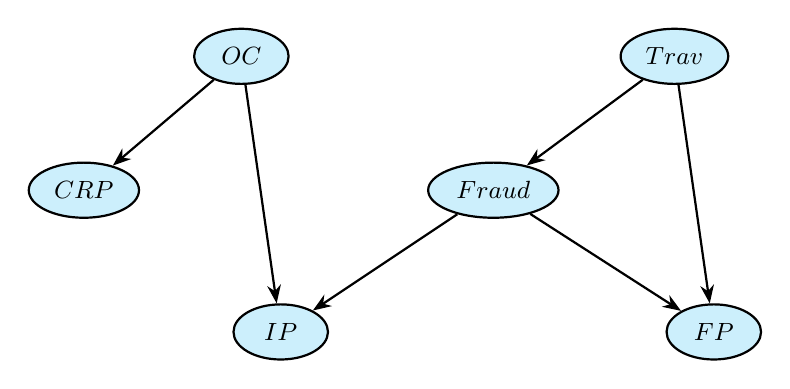
\begin{tikzpicture}[
  every node/.style={draw,ellipse,minimum width=1.2cm,
    minimum height=0.7cm,font=\small\bfseries,fill=cyan!20},
  ->,>=Stealth,thick]
  \node (OC)    at (2,   3.5) {$OC$};
  \node (Trav)  at (7.5, 3.5) {$Trav$};
  \node (CRP)   at (0,   1.8) {$CRP$};
  \node (Fraud) at (5.2, 1.8) {$Fraud$};
  \node (IP)    at (2.5, 0)   {$IP$};
  \node (FP)    at (8,   0)   {$FP$};
  \draw (OC)--(CRP); \draw (OC)--(IP);
  \draw (Trav)--(Fraud); \draw (Trav)--(FP);
  \draw (Fraud)--(IP); \draw (Fraud)--(FP);
\end{tikzpicture}
\end{center}

\[
P(\textit{Trav}{=}T)=0.05,\qquad P(\textit{OC}{=}T)=0.75
\]

\begin{center}
\begin{tabular}{ccc}
\toprule
$\textit{Trav}$ & $P(\textit{Fraud}{=}T)$ & $P(\textit{Fraud}{=}F)$\\
\midrule
T & 0.010 & 0.990\\
F & 0.004 & 0.996\\
\bottomrule
\end{tabular}
\end{center}

\begin{center}
\begin{tabular}{cccc}
\toprule
$\textit{Trav}$ & $\textit{Fraud}$ & $P(\textit{FP}{=}T)$ & $P(\textit{FP}{=}F)$\\
\midrule
T & T & 0.90 & 0.10\\
T & F & 0.90 & 0.10\\
F & T & 0.10 & 0.90\\
F & F & 0.01 & 0.99\\
\bottomrule
\end{tabular}
\quad
\begin{tabular}{cccc}
\toprule
$\textit{Fraud}$ & $\textit{OC}$ & $P(\textit{IP}{=}T)$ & $P(\textit{IP}{=}F)$\\
\midrule
T & T & 0.020 & 0.980\\
T & F & 0.011 & 0.989\\
F & T & 0.010 & 0.990\\
F & F & 0.001 & 0.999\\
\bottomrule
\end{tabular}
\quad
\begin{tabular}{ccc}
\toprule
$\textit{OC}$ & $P(\textit{CRP}{=}T)$ & $P(\textit{CRP}{=}F)$\\
\midrule
T & 0.100 & 0.900\\
F & 0.001 & 0.999\\
\bottomrule
\end{tabular}
\end{center}

Note: The FP CPT has $P(\textit{FP}{=}T\mid\textit{Trav}{=}T)=0.90$ for both values of Fraud,
because the problem states ``when the card holder is travelling, 90\% of transactions are
foreign purchases \emph{regardless of the legitimacy of the transactions}.''

\subsection*{(b) Probability Queries}

\paragraph{Query 1: $P(\textit{Fraud})$}

\begin{align*}
P(\textit{Fraud}{=}T)
  &=P(\textit{Fraud}{=}T\mid\textit{Trav}{=}T)\cdot P(\textit{Trav}{=}T)
   +P(\textit{Fraud}{=}T\mid\textit{Trav}{=}F)\cdot P(\textit{Trav}{=}F)\\
  &=0.01\times0.05+0.004\times0.95
   =0.0005+0.0038=\boxed{0.0043}
\end{align*}

Before any transaction evidence is observed, the \textbf{baseline probability of fraud is 0.43\%}.

\paragraph{Query 2: $P(\textit{Fraud}\mid\textit{FP}{=}T,\textit{IP}{=}F,\textit{CRP}{=}T)$}

With $\alpha=\tfrac{1}{P(\textit{FP}{=}T,\textit{IP}{=}F,\textit{CRP}{=}T)}$,
marginalizing over $\textit{Trav}$ and $\textit{OC}$:

\begin{align*}
P(\textit{Fraud}\mid\textit{FP},\neg\textit{IP},\textit{CRP})
&=\alpha\sum_{\textit{Trav}}P(\textit{Trav})\,P(\textit{Fraud}\mid\textit{Trav})\,
  P(\textit{FP}{=}T\mid\textit{Trav},\textit{Fraud})\\
&\hspace{30pt}\times
  \sum_{\textit{OC}}P(\textit{OC})\,P(\textit{CRP}{=}T\mid\textit{OC})\,
  P(\textit{IP}{=}F\mid\textit{Fraud},\textit{OC})
\end{align*}

First we compute the inner OC sum for each value of Fraud:
\begin{align*}
\text{OC sum (Fraud=T)}&=0.75\times0.1\times0.980+0.25\times0.001\times0.989
 =0.07350+0.000247=0.073747\\
\text{OC sum (Fraud=F)}&=0.75\times0.1\times0.990+0.25\times0.001\times0.999
 =0.07425+0.000250=0.074500
\end{align*}

\textbf{For $\textit{Fraud}=T$:}
\begin{align*}
&=\alpha\times\bigl[\underbrace{0.05\times0.01\times0.90}_{\textit{Trav}=T}
  +\underbrace{0.95\times0.004\times0.10}_{\textit{Trav}=F}\bigr]
  \times0.073747\\
&=\alpha\times(0.000450+0.000380)\times0.073747\\
&=\alpha\times0.000830\times0.073747\\
&=0.0000612\,\alpha
\end{align*}

\textbf{For $\textit{Fraud}=F$:}
\begin{align*}
&=\alpha\times\bigl[\underbrace{0.05\times0.99\times0.90}_{\textit{Trav}=T}
  +\underbrace{0.95\times0.996\times0.01}_{\textit{Trav}=F}\bigr]
  \times0.074500\\
&=\alpha\times(0.044550+0.009462)\times0.074500\\
&=\alpha\times0.054012\times0.074500\\
&=0.004024\,\alpha
\end{align*}

\paragraph{Normalization:}
\[
\alpha=\frac{1}{0.0000612+0.004024}=\frac{1}{0.004085}\approx244.8
\]
\begin{align*}
P(\textit{Fraud}{=}T\mid\textit{FP}{=}T,\textit{IP}{=}F,\textit{CRP}{=}T)
  &=244.8\times0.0000612\approx0.015\\
P(\textit{Fraud}{=}F\mid\textit{FP}{=}T,\textit{IP}{=}F,\textit{CRP}{=}T)
  &=244.8\times0.004024\approx0.985
\end{align*}
\[
\boxed{P(\textit{Fraud}\mid\textit{FP}{=}T,\textit{IP}{=}F,\textit{CRP}{=}T)
=\langle\,0.015,\;0.985\,\rangle}
\]

The probability that the transaction is fraudulent \textbf{increases from 0.43\% to approximately
1.5\%} given the evidence of a foreign purchase, no internet purchase, and a recent
computer-related accessory purchase. While the foreign purchase raises suspicion, the
overall fraud probability remains low because non-fraudulent travellers are also likely
to make foreign purchases.

\newpage
%%%%%%%%%%%%%%%%%%%%%%%%%%%%%%%%%%%%%%%%%%%%%%%%%%%
\section{Problem 4 (40 points): HMM Search and Rescue}
%%%%%%%%%%%%%%%%%%%%%%%%%%%%%%%%%%%%%%%%%%%%%%%%%%%

The rover starts at position $A$ on day 1 ($X_1=A$). Positions are
$X_t\in\{A,B,C,D,E,F\}$; the rover moves east with probability $0.8$ and
stays with probability $0.2$. Volcanic vents at $A$ and $D$ give
$P(E_t{=}\text{hot}\mid X_t\in\{A,D\})=1$ and
$P(E_t{=}\text{cold}\mid X_t\notin\{A,D\})=1$ with no noise.

\begin{center}
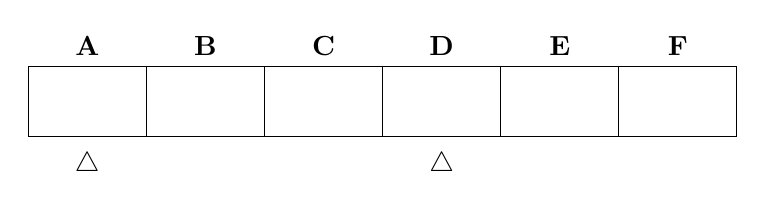
\begin{tikzpicture}
  \foreach \i/\name in {0/A,1/B,2/C,3/D,4/E,5/F}{
    \draw (\i*1.5,0) rectangle (\i*1.5+1.5,0.9);
    \node at (\i*1.5+0.75,1.15) {\textbf{\name}};
  }
  \node at (0.75,-0.35){$\bigtriangleup$};
  \node at (5.25,-0.35){$\bigtriangleup$};
\end{tikzpicture}
\end{center}

\paragraph{Transition model $P(X_{t+1}\mid X_t)$:}
Each state transitions east with $p=0.8$ or stays with $p=0.2$; $F$ is absorbing.

\begin{center}
\begin{tabular}{ccccccc}
\toprule
& A & B & C & D & E & F \\
\midrule
A & 0.2 & 0.8 & 0 & 0 & 0 & 0 \\
B & 0 & 0.2 & 0.8 & 0 & 0 & 0 \\
C & 0 & 0 & 0.2 & 0.8 & 0 & 0 \\
D & 0 & 0 & 0 & 0.2 & 0.8 & 0 \\
E & 0 & 0 & 0 & 0 & 0.2 & 0.8 \\
F & 0 & 0 & 0 & 0 & 0 & 1 \\
\bottomrule
\end{tabular}
\end{center}

\paragraph{Observation model $P(E_t\mid X_t)$:}

\begin{center}
\begin{tabular}{ccc}
\toprule
$X_t$ & $P(\text{hot})$ & $P(\text{cold})$\\
\midrule
A & 1 & 0\\
B & 0 & 1\\
C & 0 & 1\\
D & 1 & 0\\
E & 0 & 1\\
F & 0 & 1\\
\bottomrule
\end{tabular}
\end{center}

The forward filtering recurrence is:
\[
P(X_t\mid e_{1:t})\;\propto\;
P(E_t\mid X_t)\sum_{X_{t-1}}P(X_t\mid X_{t-1})\,P(X_{t-1}\mid e_{1:t-1})
\]

\paragraph{Day 1.}
$X_1=A$ with certainty; $E_1=\text{hot}$ is consistent with $A$ being a vent:
\[
P(X_1\mid E_1{=}\text{hot})=\langle1,0,0,0,0,0\rangle
\]

\paragraph{Day 2 (intermediate computation).}
Propagating forward from $X_1=A$:
\[
\sum_{X_1}P(X_2\mid X_1)\,P(X_1\mid e_1)
=\langle0.2,0.8,0,0,0,0\rangle
\]
Multiplying element-wise by $P(E_2{=}\text{cold}\mid X_2)=\langle0,1,1,0,1,1\rangle$:
\[
\propto\langle0,0.8,0,0,0,0\rangle
\]
After normalization ($\alpha=1/0.8=1.25$):
\[
P(X_2\mid e_{1:2})=\langle0,1.0,0,0,0,0\rangle
\]

\subsection*{1.\ Filtering: $P(X_3\mid\text{hot}_1,\text{cold}_2,\text{cold}_3)$}

Propagating forward from $X_2=B$ with certainty:
\[
\sum_{X_2}P(X_3\mid X_2)\,P(X_2\mid e_{1:2})
=\langle0,0.2,0.8,0,0,0\rangle
\]
Multiplying element-wise by $P(E_3{=}\text{cold}\mid X_3)=\langle0,1,1,0,1,1\rangle$:
\[
\propto\langle0,0.2,0.8,0,0,0\rangle
\]
Values sum to $1.0$; no further normalization needed.

\begin{center}
\begin{tabular}{cc}
\toprule
$X_3$ & $P(X_3\mid\text{hot}_1,\text{cold}_2,\text{cold}_3)$\\
\midrule
A & 0.0\\ B & 0.2\\ C & 0.8\\ D & 0.0\\ E & 0.0\\ F & 0.0\\
\bottomrule
\end{tabular}
\end{center}
\[
\boxed{P(X_3\mid\text{hot}_1,\text{cold}_2,\text{cold}_3)
=\langle\,0,\;0.2,\;0.8,\;0,\;0,\;0\,\rangle}
\]

After three days of observations (hot, cold, cold), the rover is most likely at
position \textbf{C with probability 0.8}, or at B with probability 0.2.

\subsection*{2.\ Smoothing: $P(X_2\mid\text{hot}_1,\text{cold}_2,\text{cold}_3)$}

Using the forward-backward algorithm:
$P(X_2\mid e_{1:3})\propto P(X_2\mid e_{1:2})\times P(e_3\mid X_2)$

First compute the backward message $P(E_3{=}\text{cold}\mid X_2)$ by summing over $X_3$:
\[
P(E_3{=}\text{cold}\mid X_2)=\sum_{X_3}P(X_3\mid X_2)\,P(E_3{=}\text{cold}\mid X_3)
\]

\begin{center}
\begin{tabular}{cl}
\toprule
$X_2$ & Computation\\
\midrule
A & $0.2\times0+0.8\times1=0.8$\\
B & $0.2\times1+0.8\times1=1.0$\\
C & $0.2\times1+0.8\times0=0.2$\\
D & $0.2\times0+0.8\times1=0.8$\\
E & $0.2\times1+0.8\times1=1.0$\\
F & $0\times1+1\times1=1.0$\\
\bottomrule
\end{tabular}
\end{center}

So the backward message is $\langle0.8,1.0,0.2,0.8,1.0,1.0\rangle$.

Since $P(X_2\mid e_{1:2})=\langle0,1,0,0,0,0\rangle$ (nonzero only at $B$):
\[
P(X_2\mid e_{1:3})\propto\langle0.8,1.0,0.2,0.8,1.0,1.0\rangle
\odot\langle0,1,0,0,0,0\rangle
=\langle0,1.0,0,0,0,0\rangle
\]

\begin{center}
\begin{tabular}{cc}
\toprule
$X_2$ & $P(X_2\mid\text{hot}_1,\text{cold}_2,\text{cold}_3)$\\
\midrule
A & 0.0\\ B & 1.0\\ C & 0.0\\ D & 0.0\\ E & 0.0\\ F & 0.0\\
\bottomrule
\end{tabular}
\end{center}
\[
\boxed{P(X_2\mid\text{hot}_1,\text{cold}_2,\text{cold}_3)
=\langle\,0,\;1.0,\;0,\;0,\;0,\;0\,\rangle}
\]

Using all three days of evidence, we can confirm with \textbf{certainty that the rover
was at position B on day 2}.

\subsection*{3.\ Prediction: $P(\text{hot}_4\mid\text{hot}_1,\text{cold}_2,\text{cold}_3)$}

We first need $P(X_4\mid e_{1:3})$ (computed in Part 4 below), then:
\[
P(\text{hot}_4\mid e_{1:3})
=\sum_{X_4}P(E_4{=}\text{hot}\mid X_4)\,P(X_4\mid e_{1:3})
\]

Only $X_4=D$ contributes since $P(\text{hot}\mid X_4)=1$ only when $X_4\in\{A,D\}$,
and from Part~4, $P(X_4{=}D\mid e_{1:3})=0.64$:
\[
=0\times0.04+0\times0.32+1\times0.64+0\times0+0\times0
=\boxed{0.64}
\]

There is a \textbf{64\% probability of observing a hot reading on day 4},
corresponding to the rover having reached vent D.

\subsection*{4.\ Prediction: $P(X_4\mid\text{hot}_1,\text{cold}_2,\text{cold}_3)$}

Propagating $P(X_3\mid e_{1:3})$ forward one step with no new evidence:
\[
P(X_4\mid e_{1:3})=\sum_{X_3}P(X_4\mid X_3)\,P(X_3\mid e_{1:3})
\]

\begin{align*}
P(X_4{=}A)&=0 \quad\text{(unreachable)}\\
P(X_4{=}B)&=P(B\mid B)\times0.2+P(B\mid C)\times0.8=0.2\times0.2+0\times0.8=0.04\\
P(X_4{=}C)&=P(C\mid B)\times0.2+P(C\mid C)\times0.8=0.8\times0.2+0.2\times0.8=0.32\\
P(X_4{=}D)&=P(D\mid B)\times0.2+P(D\mid C)\times0.8=0\times0.2+0.8\times0.8=0.64\\
P(X_4{=}E)&=0 \quad\text{(unreachable in one step from B or C)}\\
P(X_4{=}F)&=0
\end{align*}

\begin{center}
\begin{tabular}{cc}
\toprule
$X_4$ & $P(X_4\mid\text{hot}_1,\text{cold}_2,\text{cold}_3)$\\
\midrule
A & 0.00\\ B & 0.04\\ C & 0.32\\ D & 0.64\\ E & 0.00\\ F & 0.00\\
\bottomrule
\end{tabular}
\end{center}
\[
\boxed{P(X_4\mid\text{hot}_1,\text{cold}_2,\text{cold}_3)
=\langle\,0,\;0.04,\;0.32,\;0.64,\;0,\;0\,\rangle}
\]

On day 4, the rover is most likely at \textbf{position D with probability 0.64},
having traveled east from C (which itself was the most likely position on day 3).

\subsection*{Bonus (10 points):
$P(\text{hot}_4,\text{hot}_5,\text{cold}_6\mid\text{hot}_1,\text{cold}_2,\text{cold}_3)$}

We use the likelihood of future evidence given current state, working backwards:
\[
P(e_4,e_5,e_6\mid e_{1:3})
=\sum_{X_3}P(X_3\mid e_{1:3})\,P(e_{4:6}\mid X_3)
\]
where $P(e_{4:6}\mid X_3)=\sum_{X_4}P(X_4\mid X_3)\,P(e_4\mid X_4)\,P(e_{5:6}\mid X_4)$.

\textbf{Step 1 --- Compute $P(E_6{=}\text{cold}\mid X_5)$:}
\[
P(E_6{=}\text{cold}\mid X_5)=\sum_{X_6}P(X_6\mid X_5)\,P(\text{cold}\mid X_6)
\]
\begin{center}
\begin{tabular}{cl}
\toprule
$X_5$ & Computation\\
\midrule
A & $0.2\times P(\text{cold}|A)+0.8\times P(\text{cold}|B)=0.2\times0+0.8\times1=0.8$\\
B & $0.2\times1+0.8\times1=1.0$\\
C & $0.2\times1+0.8\times0=0.2$\\
D & $0.2\times0+0.8\times1=0.8$\\
E & $0.2\times1+0.8\times1=1.0$\\
F & $1\times1=1.0$\\
\bottomrule
\end{tabular}
\end{center}
\[
P(E_6{=}\text{cold}\mid X_5)=\langle0.8,1.0,0.2,0.8,1.0,1.0\rangle
\]

\textbf{Step 2 --- Compute $P(E_5{=}\text{hot},E_6{=}\text{cold}\mid X_4)$:}
\[
P(e_{5:6}\mid X_4)=\sum_{X_5}P(X_5\mid X_4)\,P(\text{hot}\mid X_5)\,P(E_6{=}\text{cold}\mid X_5)
\]
\begin{center}
\begin{tabular}{cl}
\toprule
$X_4$ & Computation\\
\midrule
A & $0.2\times P(\text{hot}|A)\times0.8+0.8\times P(\text{hot}|B)\times1.0
    =0.2\times1\times0.8+0.8\times0\times1.0=0.16$\\
B & $0.2\times0\times1.0+0.8\times0\times0.2=0$\\
C & $0.2\times0\times0.2+0.8\times1\times0.8=0.64$\\
D & $0.2\times1\times0.8+0.8\times0\times1.0=0.16$\\
E & $0.2\times0+0.8\times0=0$\\
F & $0$\\
\bottomrule
\end{tabular}
\end{center}
\[
P(e_{5:6}\mid X_4)=\langle0.16,0,0.64,0.16,0,0\rangle
\]

\textbf{Step 3 --- Compute $P(E_4{=}\text{hot},E_5{=}\text{hot},E_6{=}\text{cold}\mid X_3)$:}
\[
P(e_{4:6}\mid X_3)=\sum_{X_4}P(X_4\mid X_3)\,P(\text{hot}\mid X_4)\,P(e_{5:6}\mid X_4)
\]
\begin{center}
\begin{tabular}{cl}
\toprule
$X_3$ & Computation\\
\midrule
B & $0.2\times P(\text{hot}|B)\times0+0.8\times P(\text{hot}|C)\times0.64=0$\\
C & $0.2\times P(\text{hot}|C)\times0.64+0.8\times P(\text{hot}|D)\times0.16
    =0.2\times0\times0.64+0.8\times1\times0.16=0.128$\\
\bottomrule
\end{tabular}
\end{center}
\[
P(e_{4:6}\mid X_3)=\langle0,0,0.128,0,0,0\rangle
\quad\text{(only nonzero at }X_3{=}C\text{)}
\]

\textbf{Final combination:}
\begin{align*}
P(\text{hot}_4,\text{hot}_5,\text{cold}_6\mid e_{1:3})
&=\sum_{X_3}P(X_3\mid e_{1:3})\,P(e_{4:6}\mid X_3)\\
&=0\times0+0.2\times0+0.8\times0.128+0\times0+0\times0+0\times0\\
&=0.8\times0.128=\boxed{0.1024}
\end{align*}

The probability of observing hot, hot, cold on days 4, 5, and 6 respectively is \textbf{10.24\%}.
This requires the rover to reach vent D by day 4 (probability 0.64), stay at D on day 5
(probability 0.2), and then move to E on day 6 (probability 0.8).

\newpage
%%%%%%%%%%%%%%%%%%%%%%%%%%%%%%%%%%%%%%%%%%%%%%%%%%%
\section{Problem 5 (10 points): Markov Decision Process}
%%%%%%%%%%%%%%%%%%%%%%%%%%%%%%%%%%%%%%%%%%%%%%%%%%%

States $\{A,B\}$, actions $\{1,2\}$, discount $\gamma=1$:

\begin{center}
\begin{tabular}{cccc}
\toprule
$s$ & $a$ & $s'$ & $T(s,a,s')$\\
\midrule
A & 1 & A & 1.0\\ A & 1 & B & 0.0\\
A & 2 & A & 0.5\\ A & 2 & B & 0.5\\
B & 1 & A & 0.0\\ B & 1 & B & 1.0\\
B & 2 & A & 0.0\\ B & 2 & B & 1.0\\
\bottomrule
\end{tabular}
\qquad
\begin{tabular}{ccc}
\toprule
$s$ & $a$ & $R(s,a)$\\
\midrule
A & 1 & $\phantom{-}0$\\
A & 2 & $-1$\\
B & 1 & $\phantom{-}5$\\
B & 2 & $\phantom{-}0$\\
\bottomrule
\end{tabular}
\end{center}

\subsection*{1.\ Bellman Equation}

\[
V^{\pi}(s)=R\bigl(s,\pi(s)\bigr)+\gamma\sum_{s'}T\bigl(s,\pi(s),s'\bigr)\,V^{\pi}(s')
\]

With $\gamma=1$ this simplifies to:
\[
V^{\pi}(s)=R\bigl(s,\pi(s)\bigr)+\sum_{s'}T\bigl(s,\pi(s),s'\bigr)\,V^{\pi}(s')
\]

\subsection*{2.\ Two Iterations of Policy Evaluation ($\pi(A)=1,\;\pi(B)=1$)}

Initialize $V^{\pi}_0(A)=V^{\pi}_0(B)=0$.

\textbf{Iteration 1:}
\begin{align*}
V^{\pi}_1(A)&=R(A,1)+T(A,1,A)\,V^{\pi}_0(A)+T(A,1,B)\,V^{\pi}_0(B)
             =0+1\times0+0\times0=0\\
V^{\pi}_1(B)&=R(B,1)+T(B,1,A)\,V^{\pi}_0(A)+T(B,1,B)\,V^{\pi}_0(B)
             =5+0\times0+1\times0=5
\end{align*}

\textbf{Iteration 2:}
\begin{align*}
V^{\pi}_2(A)&=R(A,1)+T(A,1,A)\,V^{\pi}_1(A)+T(A,1,B)\,V^{\pi}_1(B)
             =0+1\times0+0\times5=\boxed{0}\\
V^{\pi}_2(B)&=R(B,1)+T(B,1,A)\,V^{\pi}_1(A)+T(B,1,B)\,V^{\pi}_1(B)
             =5+0\times0+1\times5=\boxed{10}
\end{align*}

After two iterations, $V^{\pi}_2(A)=0$ and $V^{\pi}_2(B)=10$.

\subsection*{3.\ Policy Improvement}

\[
\pi_{\text{new}}(s)=\arg\max_{a}\Bigl[R(s,a)+\sum_{s'}T(s,a,s')\,V^{\pi}_2(s')\Bigr]
\]

\textbf{State $A$:}
\begin{align*}
a=1:&\quad 0+1\times0+0\times10=0\\
a=2:&\quad -1+0.5\times0+0.5\times10=4
\end{align*}
Since $4>0$, set $\pi_{\text{new}}(A)=2$.

\textbf{State $B$:}
\begin{align*}
a=1:&\quad 5+0\times0+1\times10=15\\
a=2:&\quad 0+0\times0+1\times10=10
\end{align*}
Since $15>10$, set $\pi_{\text{new}}(B)=1$.

\[
\boxed{\pi_{\text{new}}(A)=2,\qquad\pi_{\text{new}}(B)=1}
\]

The improved policy \textbf{switches state $A$ from action 1 to action 2}: staying at $A$
forever (action 1) yields value 0, whereas action 2 gives a 50\% chance of reaching $B$
each step, which has value 10, making the expected return $-1+0.5\times10=4>0$.
State $B$ retains action 1, as it yields $5+10=15$ versus action 2's $0+10=10$.

\end{document}
